%==============================================================================
% SIMTiX — M.Tech. Thesis
% A Compact Open-Source RISC-V SIMT Accelerator, its Floating-Point Extension,
% and an End-to-End Quantized (INT8) Neural-Network Inference Engine.
%
% Build:  pdflatex simtix_thesis && pdflatex simtix_thesis && pdflatex simtix_thesis
%         (three passes resolve the ToC, list of figures/tables, and references)
%==============================================================================
\documentclass[12pt,a4paper,oneside]{report}

\usepackage[T1]{fontenc}
\usepackage[utf8]{inputenc}
\usepackage{newtxtext,newtxmath}          % Times-like professional serif + math
\usepackage[a4paper,inner=1.4in,outer=1.0in,top=1.0in,bottom=1.0in]{geometry}
\usepackage{setspace}
\onehalfspacing
\usepackage{graphicx}
\graphicspath{{../figs/}{../../ml/data/}}
\usepackage{rotating}                      % sidewaysfigure for the chip_top diagram
\usepackage{amsmath}
\let\Bbbk\relax                            % avoid newtxmath/amssymb \Bbbk clash
\usepackage{amssymb}
\usepackage{booktabs}
\usepackage{array}
\usepackage{multirow}
\usepackage{siunitx}
\usepackage{xcolor}
\usepackage{listings}
\usepackage{caption}
\captionsetup{font=small,labelfont=bf,skip=6pt}
\usepackage[hidelinks]{hyperref}
\usepackage{fancyhdr}
\usepackage{emptypage}
\usepackage{titlesec}

% --- section / chapter styling -----------------------------------------------
\titleformat{\chapter}[display]
  {\normalfont\huge\bfseries}{\chaptertitlename\ \thechapter}{16pt}{\Huge}
\titlespacing*{\chapter}{0pt}{0pt}{24pt}

% --- running headers ---------------------------------------------------------
\pagestyle{fancy}
\fancyhf{}
\renewcommand{\headrulewidth}{0.4pt}
\fancyhead[L]{\small\nouppercase{\leftmark}}
\fancyhead[R]{\small\thepage}
\renewcommand{\chaptermark}[1]{\markboth{\thechapter.\ #1}{}}

% --- code listing style ------------------------------------------------------
\definecolor{codegray}{gray}{0.95}
\lstset{
  basicstyle=\ttfamily\small,
  columns=fullflexible,
  keepspaces=true,
  breaklines=true,
  frame=single,
  framesep=4pt,
  backgroundcolor=\color{codegray},
  numbers=none,
  aboveskip=8pt, belowskip=8pt,
  captionpos=b,
  showstringspaces=false
}

\newcommand{\code}[1]{\texttt{#1}}
\sisetup{group-separator={,},group-minimum-digits=4}

\begin{document}

%==============================================================================
% TITLE PAGE
%==============================================================================
\begin{titlepage}
\centering
\vspace*{0.5cm}
{\large\scshape Indian Institute of Technology Mandi\par}
\vspace{2.0cm}
{\Large\bfseries SIMTiX:\\[0.3em]
A Compact Open-Source RISC-V SIMT Accelerator and its Extension\\
into an End-to-End Quantized Neural-Network Inference Engine\par}
\vspace{2.0cm}
{\large A thesis submitted in partial fulfillment of the requirements\\
for the degree of\par}
\vspace{0.4cm}
{\large\bfseries Master of Technology\par}
\vspace{2.0cm}
{\large\itshape by\par}
\vspace{0.4cm}
{\Large\bfseries Krishna Gorai\par}
\vspace{3.0cm}
{\large School of Computing and Electrical Engineering\\
Indian Institute of Technology Mandi\par}
\vspace{1.5cm}
{\large 2026\par}
\end{titlepage}

%==============================================================================
% DECLARATION
%==============================================================================
\pagenumbering{roman}
\chapter*{Declaration}
\addcontentsline{toc}{chapter}{Declaration}
\thispagestyle{plain}

I declare that the work presented in this thesis, titled \emph{``SIMTiX: A
Compact Open-Source RISC-V SIMT Accelerator and its Extension into an End-to-End
Quantized Neural-Network Inference Engine,''} is my own. The register-transfer
level (RTL) design, the verification testbenches, the kernels, the field-programmable
gate array (FPGA) implementation flow, and the software model reported here were
developed by me. Every quantitative result stated in this thesis was obtained by
running the corresponding simulation or implementation flow on the design; no
figure has been estimated or reproduced from another source except where it is
explicitly cited or explicitly labelled as an estimate. The complete source,
including the RTL, the simulation harness, and the FPGA scripts, is publicly
available.

\vspace{2.5cm}
\noindent Krishna Gorai\\
Indian Institute of Technology Mandi

\clearpage

%==============================================================================
% ABSTRACT
%==============================================================================
\chapter*{Abstract}
\addcontentsline{toc}{chapter}{Abstract}
\thispagestyle{plain}

This thesis presents \textbf{SIMTiX}, a compact, fully open-source
Single-Instruction Multiple-Thread (SIMT) accelerator for RISC-V, and its
evolution from a general-purpose parallel core into an end-to-end quantized
neural-network inference engine. The work is developed as a continuous
engineering narrative in which every design decision is measured rather than
asserted.

The baseline accelerator implements the complete SIMT mechanism set in a small,
readable, synthesizable design: eight lanes organised into hardware warps, a
round-robin scheduler with a background memory engine for latency hiding,
address coalescing on a cache-line-wide data port, a per-warp reconvergence
stack for control divergence, and an on-chip scratchpad for data reuse. It is
attached to a reused five-stage RISC-V host through a memory-mapped offload
interface and taken through the entire flow from RTL to a routed FPGA bitstream
on a Xilinx Zynq UltraScale+ device. A central implementation result is that
placing the vector register file and scratchpad in distributed RAM (LUTRAM)
reduces the design from \SI{74}{\percent} to \SI{13}{\percent} of the device
LUTs while closing timing at \SI{100}{\mega\hertz}. A six-kernel benchmark suite,
verified bit-exact to 1024 threads, gives a measured $7$--$10\times$ speedup over
the scalar host on streaming kernels and---reported honestly---a slowdown on a
serial reduction, mapping precisely where the SIMT model does and does not pay.

The accelerator is then extended with a per-lane floating-point unit supporting
both single (FP32) and half (FP16) precision, including the fused multiply-add
and iterative divide and square root, verified bit-exact against an IEEE-754
reference over \num{116089} vectors. A placed timing-closure study localises the
frequency bottleneck to a single lane's fused-multiply-add cone and, by
pipelining it into three stages, meets \SI{100}{\mega\hertz} and moves the
critical path off the floating-point datapath; the complete system-on-chip signs
off at \SI{103.7}{\mega\hertz} as a deployable bitstream.

The final and principal contribution turns SIMTiX into an AI inference
accelerator. A custom INT8 packed dot-product instruction, \code{pdot8}, is
added as a pipelined DSP background engine that costs \num{32} additional DSP
blocks and about \SI{1}{\percent} of the LUTs while leaving the operating
frequency unregressed. On top of it, quantized GEMM and GEMV kernels and an
INT32-to-INT8 requantization step complete the operator set for a fully-connected
network. These are composed into a trained, quantized $784{\rightarrow}128{\rightarrow}10$
multilayer perceptron that classifies MNIST handwritten digits. The network runs
end-to-end on the integrated chip: the host CPU streams the weights out of an
on-chip block-RAM store into the accelerator's working memory in tiles, launches
the kernels over the memory-mapped interface, and reads back the predicted digit.
The chip reproduces the integer-exact software golden on all 64 test images,
bit-for-bit, demonstrating a programmable RISC-V SIMT core that performs real,
trained, quantized inference on measured hardware.

\clearpage

%==============================================================================
% TABLE OF CONTENTS / LISTS
%==============================================================================
\tableofcontents
\clearpage
\listoffigures
\addcontentsline{toc}{chapter}{List of Figures}
\clearpage
\listoftables
\addcontentsline{toc}{chapter}{List of Tables}
\clearpage

%==============================================================================
% BODY
%==============================================================================
\pagenumbering{arabic}

%------------------------------------------------------------------------------
\chapter{Introduction}
\label{ch:intro}
%------------------------------------------------------------------------------

\section{Motivation}
Graphics processing units (GPUs) execute thousands of scalar threads in lockstep
groups called \emph{warps} under a Single-Instruction Multiple-Thread (SIMT)
model. The microarchitectural mechanisms that make this efficient---warp
scheduling for latency hiding, memory coalescing, control-divergence handling,
and on-chip scratchpads---are well documented at the level of commercial GPUs,
but they are hard to \emph{study in register-transfer level (RTL) form}.
Production GPUs are proprietary; open GPGPU cores such as Vortex are powerful but
large and difficult to bring up; and small academic cores are often
simulator-only, stopping short of a real implementation flow. There is a gap
between a design that is small enough to read end-to-end and one that is complete
enough to run a real workload on real hardware.

At the same time, the dominant workload for accelerators has shifted to neural
network inference, and inference no longer runs in floating point. It runs in
\emph{quantized integer} arithmetic---most commonly INT8---because four INT8
values pack into one 32-bit word, quadrupling both the effective memory bandwidth
and the arithmetic density of a datapath, while post-training quantization holds
accuracy within a fraction of a percent of the floating-point reference. A
credible accelerator today must therefore express low-precision arithmetic
efficiently and demonstrate it on a real network.

This thesis addresses both gaps with a single design. It builds a compact,
fully-open SIMT accelerator whose entire path---RTL, simulation, synthesis,
place-and-route, and a routed bitstream---is reproducible on one workstation with
free or widely available tools, and it then extends that accelerator, step by
measured step, into an engine that performs end-to-end quantized neural-network
inference. The design is small enough to be read as a teaching artefact yet
complete enough that a trained network runs on it and produces correct answers on
measured silicon-class hardware.

\section{Objectives}
The thesis pursues four concrete objectives:
\begin{enumerate}
\item Design a complete, synthesizable SIMT accelerator---warp scheduling,
latency hiding, memory coalescing, a reconvergence stack, and a scratchpad---and
integrate it with a five-stage RISC-V host as a self-contained system-on-chip
(SoC) that is taken all the way to a routed FPGA bitstream.
\item Establish, by measurement, the FPGA cost and performance of the design,
including the implementation insight that a distributed-RAM register file, rather
than the arithmetic units, is what makes a SIMT datapath small and fast on FPGA.
\item Extend the engine with a per-lane floating-point unit in both single and
half precision, verify it bit-exact against an IEEE-754 reference, and close its
timing to \SI{100}{\mega\hertz} through a diagnosis-driven pipelining of the
fused multiply-add.
\item Turn the accelerator into an AI inference engine by adding an INT8
dot-product instruction, quantized GEMM/GEMV and requantization kernels, and a
complete on-chip demonstration of a trained, quantized MNIST classifier running
end-to-end through the real chip datapath.
\end{enumerate}

\section{Contributions}
The specific contributions, each backed by a measured result in this thesis, are:
\begin{itemize}
\item A compact, fully-open SIMT accelerator (eight lanes, four resident warps)
integrated with a five-stage RISC-V host as a self-contained SoC, exercising the
entire RTL-to-bitstream flow (Chapters~\ref{ch:arch}--\ref{ch:impl}).
\item An implementation study showing that moving the vector register file and
scratchpad into distributed RAM reduces LUT usage by $5.7\times$ and closes
\SI{100}{\mega\hertz} timing, with an analysis of why the register-file read
multiplexer, not the ALUs, dominates a naive SIMT datapath (Chapter~\ref{ch:impl}).
\item A six-kernel benchmark suite, verified bit-exact at up to 1024 threads,
that isolates distinct microarchitectural behaviours, and a measured speedup over
the scalar host---including a deliberately reported case where SIMT loses
(Chapter~\ref{ch:impl}).
\item A per-lane floating-point extension covering FP32 and FP16, in which half
precision is obtained almost for free from the single-precision path by NaN-boxed
widen--compute--narrow, verified bit-exact and closed to a deployable
\SI{103.7}{\mega\hertz} SoC by a diagnosis-driven three-stage FMA pipeline
(Chapter~\ref{ch:fp}).
\item A custom INT8 packed dot-product instruction (\code{pdot8}) implemented as
a pipelined DSP background engine that adds INT8 throughput without regressing
frequency, and a quantized operator library (GEMM, GEMV, requantization) built on
it (Chapters~\ref{ch:pdot8}--\ref{ch:requant}).
\item An end-to-end, on-chip quantized MNIST inference engine in which the host
CPU streams weights from block RAM into the accelerator's working memory in
tiles, and the integrated chip reproduces the integer-exact golden on all 64 test
images bit-for-bit (Chapter~\ref{ch:mnist}).
\end{itemize}

\section{Organisation of the thesis}
Chapter~\ref{ch:background} reviews the SIMT execution model, the RISC-V host, and
INT8 quantization. Chapter~\ref{ch:arch} describes the baseline SIMTiX
architecture in detail. Chapter~\ref{ch:impl} presents the FPGA implementation,
the LUTRAM result, and the benchmark evaluation. Chapter~\ref{ch:fp} develops the
floating-point extension and its timing-closure study. Chapter~\ref{ch:pdot8}
introduces the \code{pdot8} INT8 instruction; Chapter~\ref{ch:gemm} builds the
quantized GEMM and GEMV kernels on it; Chapter~\ref{ch:requant} adds
requantization. Chapter~\ref{ch:mnist} composes these into the end-to-end on-chip
MNIST inference engine---the capstone. Chapter~\ref{ch:results} consolidates and
discusses all results, and Chapter~\ref{ch:conclusion} concludes.

%------------------------------------------------------------------------------
\chapter{Background}
\label{ch:background}
%------------------------------------------------------------------------------

\section{The SIMT execution model}
A SIMT machine groups scalar \emph{threads} into \emph{warps} that share a single
instruction stream and execute on a vector of \emph{lanes}. SIMTiX uses a warp
size equal to its lane count ($\mathrm{WARP\_SIZE}=\mathrm{NUM\_LANES}=8$), so one
warp occupies all lanes for one instruction. Several warps are resident at once
($\mathrm{NUM\_WARPS}=4$) and time-share one fetch/decode/execute datapath; when
one warp stalls on memory, the scheduler issues another, hiding the latency.
Three effects determine SIMT efficiency:
\begin{itemize}
\item \textbf{Occupancy}: there must be enough resident warps to keep the
datapath busy while others wait on memory.
\item \textbf{Memory coalescing}: the lanes' individual memory accesses are
merged into wide transactions where they are contiguous, so that a warp's load of
adjacent addresses costs one transaction rather than eight.
\item \textbf{Control divergence}: when lanes of one warp take different branch
outcomes, the divergent paths must be serialized, which lowers the fraction of
lanes doing useful work.
\end{itemize}
SIMTiX implements hardware for all three and instruments each so it can be
measured directly.

\section{The RISC-V host and the offload model}
The accelerator is not a standalone processor; it is an \emph{offload} engine
attached to a host CPU, exactly as a discrete GPU is mapped into a host's
physical address space. The host is a reused, unmodified five-stage RISC-V
(RV32I) pipeline. Its only attach point is the data-memory interface: a single
address decode routes accesses either to the CPU's local memory or to the
accelerator's memory-mapped register page. A stock RISC-V program therefore
drives the accelerator with ordinary load and store instructions---it programs a
command block (kernel entry address, base pointers, thread count), writes a
\code{GO} bit, and polls a \code{DONE} bit. No custom host instructions are
required for control.

\section{INT8 quantization for inference}
A quantized neural network represents activations and weights as low-precision
integers instead of floating-point numbers. Under \emph{symmetric per-tensor}
quantization, a real tensor $x$ is mapped to signed 8-bit integers by a single
scale factor $S$: $x \approx S\cdot q$, with $q\in[-127,127]$. A layer then
computes its dot products in the integer domain, accumulating products of INT8
operands into a wide INT32 accumulator that never saturates for realistic
reduction lengths. To feed the \emph{next} INT8 layer, the INT32 accumulator must
be rescaled back to a signed byte---\emph{requantization}:
\begin{equation}
\mathrm{out} = \mathrm{clamp}\big(\,\mathrm{round}(\mathrm{acc}\cdot \mathit{scale} + \mathit{zp}),\,-128,\,127\big),
\label{eq:requant}
\end{equation}
where $\mathit{scale}=(S_{\text{in}}\,S_{\text{weight}})/S_{\text{out}}$ composes
the input, weight, and output scales, and $\mathit{zp}$ is a zero point (zero for
symmetric quantization). The attraction of INT8 is fourfold data density (four
bytes per 32-bit word), fourfold compute density relative to FP32 for the same
register pressure, and a mapping of the multiplies onto the FPGA's hard DSP
blocks---at a typical accuracy loss well below one percent. Chapters~\ref{ch:pdot8}
through \ref{ch:mnist} build precisely this arithmetic into SIMTiX.

%------------------------------------------------------------------------------
\chapter{The SIMTiX Architecture}
\label{ch:arch}
%------------------------------------------------------------------------------

The entire SIMT engine lives in one module, \code{warp\_pool.sv}: the scheduler,
lanes, register file, reconvergence stack, memory engine, and scratchpad are
tightly co-designed and share a single decode datapath and a single data port, so
they are implemented together rather than as separate blocks. This chapter
describes that engine as it exists in the RTL.

\section{System view and the offload interface}
The host's data-memory signals---write-enable, \code{funct3}, the ALU result used
as the address, and the write data---form the bus into the accelerator. A one-line
address decode on the address selects between the CPU's local data memory and the
accelerator's memory-mapped I/O (MMIO) page, and the read-data return is muxed
back the same way. The SoC boundary also exposes the accelerator's shared-memory
master ports: kernel code is fetched over an instruction port, and data arrays
are accessed over a cache-line-wide data port.

\begin{table}[t]
\caption{Memory-mapped command/status register map. Base address
\code{0x8000\_0000}, one 4~KB page.}
\label{tab:mmio}
\centering
\small
\begin{tabular}{lll p{6.6cm}}
\toprule
Offset & Name & R/W & Description\\
\midrule
\code{0x00} & \code{KERNEL\_PC} & W & byte address of the kernel's first instruction\\
\code{0x04} & \code{BASE\_A} & W & base pointer, argument 0\\
\code{0x08} & \code{BASE\_B} & W & base pointer, argument 1\\
\code{0x0C} & \code{BASE\_C} & W & base pointer, argument 2\\
\code{0x10} & \code{N} & W & total thread count (grid size) to launch\\
\code{0x14} & \code{CTRL} & W & bit\,0 $=$ \code{GO} (write 1 to launch)\\
\code{0x18} & \code{STATUS} & R & bit\,0 $=$ \code{DONE}, bit\,1 $=$ \code{BUSY}\\
\code{0x1C} & \code{CYCLES} & R & cycle count of the last kernel\\
\bottomrule
\end{tabular}
\end{table}

Table~\ref{tab:mmio} lists the MMIO register map. Writing \code{GO} produces a
one-cycle launch pulse; a small dispatcher finite-state machine
(\code{D\_IDLE}$\rightarrow$\code{D\_LAUNCH}$\rightarrow$\code{D\_RUN}$\rightarrow$\code{D\_DONE})
hands the whole grid to the warp pool in a single launch, counts cycles until the
pool retires it, and latches the runtime into the \code{CYCLES} register. On
\code{GO} the accelerator launches a grid of $N$ threads as $\lceil N/8\rceil$
warps; each thread receives its identity and arguments through a register-seeding
convention at spawn (\code{a0}$=$thread id, \code{a1..a3}$=$base pointers,
\code{a4}$=N$).

\begin{sidewaysfigure}
\centering
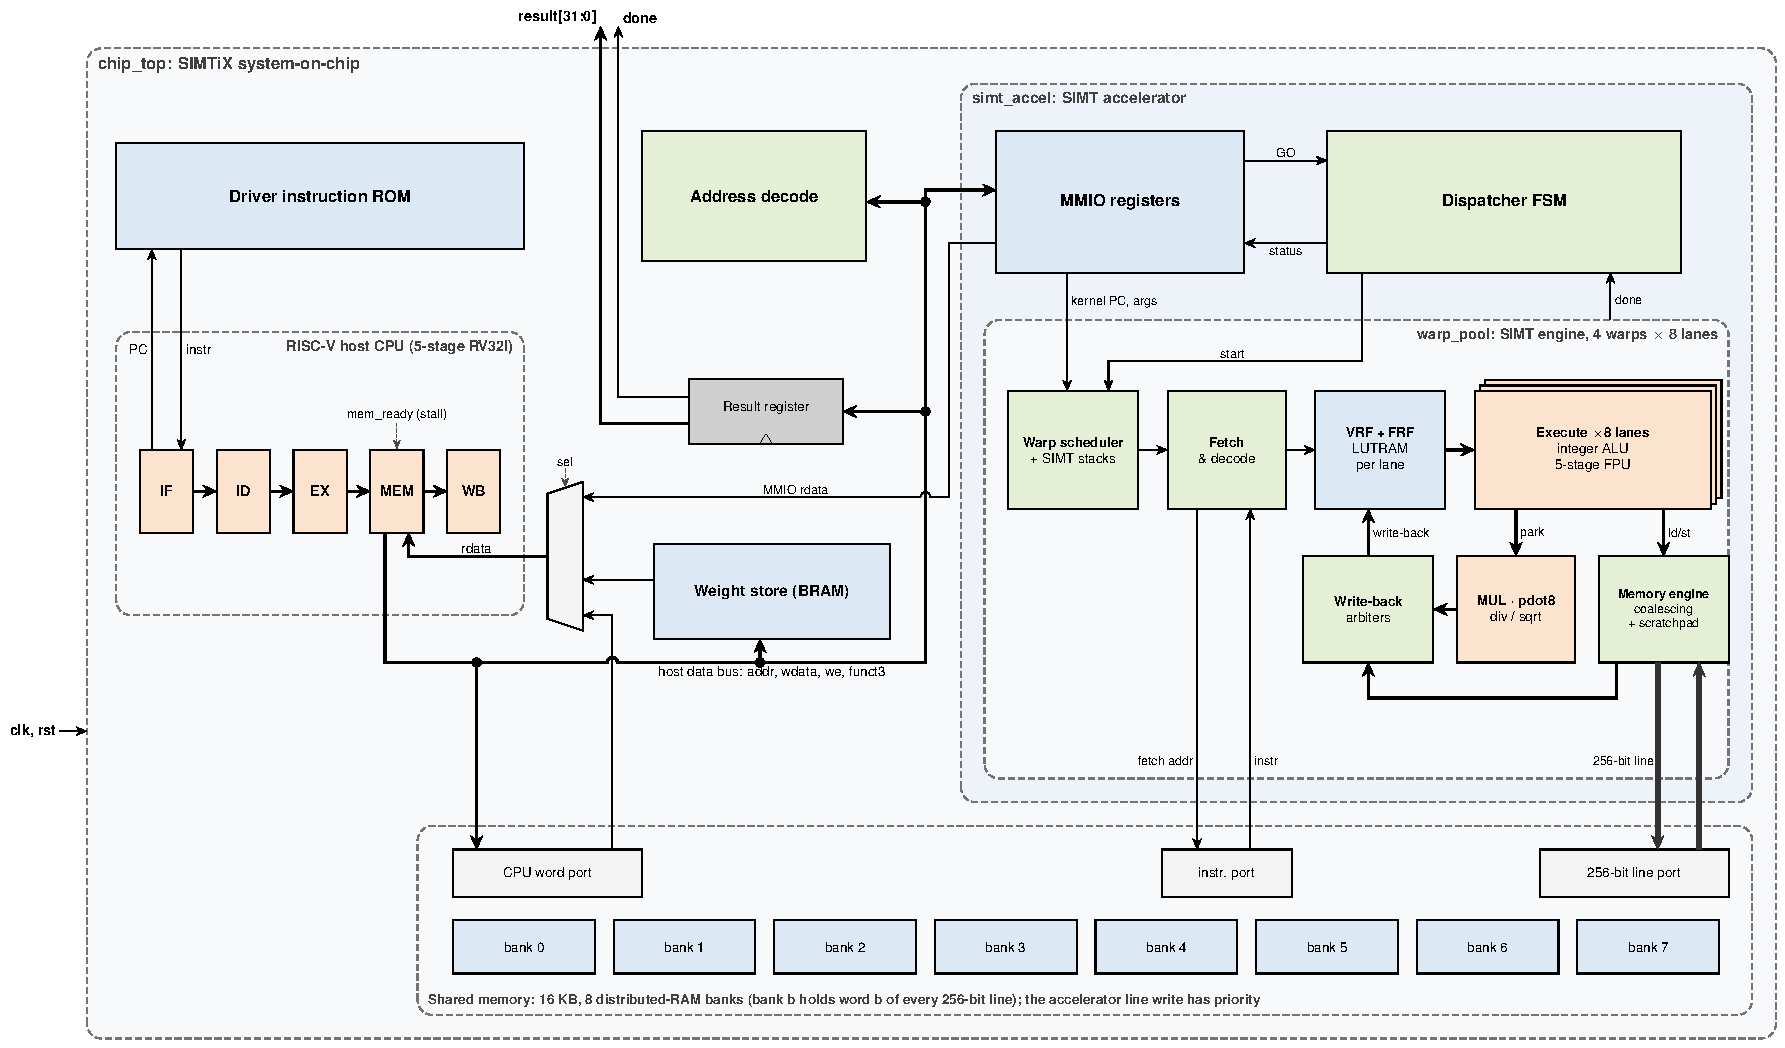
\includegraphics[width=\textwidth,height=0.88\textheight,keepaspectratio]{simtix_chip_top.pdf}
\caption{The complete SIMTiX system-on-chip, \code{chip\_top}, drawn from the RTL.
The five-stage RV32I host drives one data bus; an address decode on the top four
address bits selects the accelerator's MMIO registers, the chip result register,
the block-RAM weight store, or the shared memory, and a read-data multiplexer
returns the addressed word. Inside \code{simt\_accel}, \code{GO} starts the
dispatcher, which launches \code{warp\_pool} and counts cycles until the grid
retires. \code{warp\_pool} fetches kernel code through the shared memory's
instruction port and moves data one 256-bit line at a time through its line port.
The configuration shown is the one used for MNIST (Chapter~\ref{ch:mnist}): a
16~KB shared memory and the weight store with its one-cycle CPU stall; the
baseline chip of Chapter~\ref{ch:impl} has a 4~KB shared memory.}
\label{fig:arch}
\end{sidewaysfigure}

\section{The warp pool}
Four warp slots are resident at once (Figure~\ref{fig:arch}). Each owns private
architectural state---program counter, active mask, register-file partition, and
reconvergence stack---and all slots share one fetch/decode/ALU datapath and one
data port. A round-robin scheduler issues one runnable warp per cycle while a
background memory engine advances one coalesced transaction per cycle, so one
warp's memory latency is overlapped with other warps' compute.

\subsection{Scheduling and spawning}
Two combinational selectors run each cycle. The \emph{issue} selector scans from a
rotating pointer for the first runnable slot and issues it, then advances the
pointer (round-robin). The \emph{fill} selector scans for the first empty or
retired slot and, if grid threads remain to be spawned, drops a new warp into it:
its base thread id, a fresh base stack frame, and its active mask (a tail mask
handles a partial final warp when $N$ is not a multiple of eight). Slots are
recycled the instant a warp retires, so grids with far more warps than the four
hardware slots run correctly---this is exactly the mechanism that later lets a
single launch of $N=128$ threads run the MNIST layers.

\subsection{Fetch, decode, and the live top-of-stack view}
The top-of-stack (TOS) frame of the issuing warp gives the cycle's live view: its
current PC drives the shared instruction fetch, and its active mask says which
lanes execute. Decode is plain combinational RV32I---opcode, register fields,
\code{funct3}, the immediate forms, and the load/store/\code{ecall} flags---with
the 4-bit ALU control reused from the host core and extended for the RV32M
\code{mul}. When a pushed stack frame's PC reaches its recorded reconvergence PC,
that issue slot pops the frame instead of executing, which is how divergent lane
groups rejoin.

\subsection{Per-lane datapath}
For the issuing warp, all eight lanes evaluate in parallel each cycle. Per lane:
the two operands are read from the register file; the ALU inputs are selected by
opcode; the ALU result is computed (and doubles as the effective address for
memory operations); and a writeback value and enable are formed. Writeback is
gated off for a destination of \code{x0} and for lanes not in the active
mask---masked-off lanes make no architectural change. Branch decisions are per
lane, producing a taken mask; uniform decisions such as a jump target use the
lowest active lane as the leader.

\subsection{Control divergence: the reconvergence stack}
\label{sec:reconv}
Each warp owns a reconvergence stack of depth eight. A branch is resolved against
the active mask. If all active lanes agree, the PC is simply retargeted---no
divergence. If they disagree, the warp records the union mask at the join and
pushes a ``continue'' frame so the two lane groups run in turn:
\begin{itemize}
\item a \emph{forward} branch (a single-sided \code{if}) reconverges at the branch
target, and the pushed frame runs the fall-through lanes first;
\item a \emph{backward} branch (a loop) reconverges at the fall-through (the loop
exit), and the pushed frame runs the still-looping lanes.
\end{itemize}
The pushed frame pops when its PC reaches the recorded join, and the warp
reconverges into the frame below, which already holds the union mask. The base
frame never pops. Nesting works to the stack depth. The convention is
compiler-free: general two-sided \code{if/else} is written as two single-sided
\code{if}s. This mechanism is what keeps a data-dependent kernel such as the
Collatz step-count correct while lanes finish at different times.

\subsection{The vector register file in distributed RAM}
\label{sec:vrf}
The vector register file (VRF) is logically $\mathrm{NUM\_WARPS}\times
\mathrm{NUM\_LANES}\times 32$ 32-bit words. It is built as eight independent
per-lane banks, each a distributed-RAM array with one synchronous write port and
two asynchronous read ports, addressed by \{warp, register\}. Two mechanisms
preserve the original flip-flop semantics exactly while keeping a single write
port. First, \emph{seed-on-read}: a per-(warp, lane, register) valid bit records
whether a register has been written this grid; an unwritten register returns its
spawn seed (\code{a0}$=$thread id, \code{a1..a4}$=$arguments, else zero), which
reproduces the old ``zero the file on spawn, then seed the arguments'' behaviour
with no clearing cycle. Second, an \emph{arbitrated single write port}: the two
producers that can target the file in one cycle---the issue stage's compute
writeback and the memory engine's load writeback---are arbitrated so that at most
one writes each lane per cycle, with the memory writeback taking priority and the
compute writeback deferring (and harmlessly re-issuing) on a collision. As
Chapter~\ref{ch:impl} shows, this single design decision is what makes SIMTiX
small and fast on FPGA.

\subsection{The background memory engine and coalescing}
\label{sec:coalesce}
At most one memory instruction is in flight, because there is a single data port.
When an issuing warp executes a load or store and the engine is free, the access
context is \emph{latched}---each lane's effective address and store data, the
active mask, and the resume PC---and the warp moves to a memory-wait state.
Latching is essential because the live decode keeps tracking the currently-issued
warp, not the one being replayed. The data port is a whole 256-bit line (eight
words). Each cycle the engine picks the line of the lowest still-pending lane,
gathers every pending lane that shares that line into one transaction, extracts or
merges each lane's word, and clears those lanes; when the mask drains it writes
the resume PC back and returns the warp to the run state. The cost is the number
of distinct lines touched: a contiguous warp access collapses to one transaction,
a fully scattered one costs up to eight. A debug counter records line
transactions, making coalescing efficiency directly measurable.

\subsection{The scratchpad}
A per-warp scratchpad of 64 words occupies a dedicated address aperture; accesses
that fall in the aperture are serviced from on-chip RAM and never reach the global
data port. Data reused across a warp's lanes---for example a broadcast matrix
row---can be staged once and reused, cutting global traffic. The scratchpad is
shared across a warp's lanes and held in a single distributed-RAM array with one
read and one write port, so the engine serializes one lane per cycle; the
semantics remain exact because within one SIMT memory instruction all lanes
perform the same operation.

\subsection{Divergence-aware lane clock-gating}
\label{sec:gating}
The active mask is exactly the set of lanes doing useful work; masked-off lanes
produce no architectural change yet, in a baseline design, still clock their
pipeline registers. Treating the active mask as a per-lane clock-enable, the
lane-datapath dynamic energy that a gated design saves over a kernel is
\begin{equation}
E_{\text{saved}} = 1 - \frac{\sum_i a_i}{L\cdot\sum_i 1}
= 1 - \frac{\text{active-lane instructions}}{L\cdot\text{issued instructions}},
\label{eq:energy}
\end{equation}
where an issued instruction activates $a$ of $L$ lanes. Two hardware
counters---issued instructions and summed active lanes---make
Eq.~\eqref{eq:energy} directly observable; Chapter~\ref{ch:impl} reports the
saving as a function of divergence.

\section{Parameters}
Table~\ref{tab:params} lists the design parameters. All are set at elaboration, so
the lane count and resident-warp count can be swept, a fact the design-space
explorations of Chapters~\ref{ch:impl} and~\ref{ch:fp} exploit.

\begin{table}[t]
\caption{Principal design parameters (defaults).}
\label{tab:params}
\centering
\small
\begin{tabular}{lll}
\toprule
Parameter & Default & Meaning\\
\midrule
\code{XLEN} & 32 & data width (RV32)\\
\code{NUM\_LANES} & 8 & physical SIMT lanes\\
\code{WARP\_SIZE} & 8 & threads per warp\\
\code{NUM\_WARPS} & 4 & resident warp slots (power of two)\\
\code{SDEPTH} & 8 & reconvergence-stack depth\\
\code{LINE\_WORDS} & 8 & words per coalesced line (256-bit)\\
\code{SCRATCH\_WORDS} & 64 & scratchpad words per warp\\
\code{MMIO\_BASE} & \code{0x8000\_0000} & command-register aperture\\
\code{SCRATCH\_BASE} & \code{0x4000\_0000} & scratchpad aperture\\
\bottomrule
\end{tabular}
\end{table}

%------------------------------------------------------------------------------
\chapter{FPGA Implementation and Baseline Evaluation}
\label{ch:impl}
%------------------------------------------------------------------------------

SIMTiX is written in synthesizable SystemVerilog and integrated with the reused
five-stage RV32I host into a self-contained chip, \code{chip\_top}: host core,
driver ROM, accelerator, and an eight-bank on-chip shared memory. In the
integrated chip the host loads the operands into shared memory, launches the
accelerator, reads the results back, and publishes a checksum---so the whole
CPU$\rightarrow$memory$\rightarrow$accelerator$\rightarrow$memory$\rightarrow$CPU
loop runs in hardware. All FPGA numbers in this thesis target the Xilinx Zynq
UltraScale+ \code{xczu7ev} (\num{230400} LUTs, \num{460800} flip-flops, \num{1728}
DSP48E2 blocks).

\section{From flip-flops to distributed RAM}
\label{sec:lutram}
The first synthesis of the accelerator with a flip-flop register file consumed
\SI{170868}{} LUTs---\SI{74}{\percent} of the device---at only \SI{10}{\percent}
of its flip-flops, and topped out near \SI{122}{\mega\hertz}. The cause is
structural rather than arithmetic. A flip-flop VRF of $4\times8\times32$ 32-bit
words is \num{32768} registers read as \code{vrf[warp][lane][reg]} with
\emph{both} the warp and the register index variable, i.e.\ a 128-to-1
multiplexer per lane per read port. That multiplexer fabric, not the ALUs,
dominates the area and sets the critical path. Re-expressing the VRF as one
distributed-RAM bank per lane (Section~\ref{sec:vrf}), and likewise moving the
scratchpad into LUTRAM, removes essentially all of those registers.
Table~\ref{tab:ppa_base} quantifies the effect: the LUTs fall by $5.7\times$
(\SI{74}{\percent} to \SI{13}{\percent} of the device) and the design closes
\SI{100}{\mega\hertz} timing with positive slack. This is the single most
important implementation result of the baseline: the register file, not the
compute, is the cost of a SIMT datapath on FPGA, and distributed RAM is the lever.

\begin{table}[t]
\caption{Accelerator PPA on \code{xczu7ev} before and after moving the vector
register file and scratchpad to distributed RAM (out-of-context synthesis).}
\label{tab:ppa_base}
\centering
\small
\begin{tabular}{lrrr}
\toprule
 & FF-based VRF & \multicolumn{2}{c}{LUTRAM VRF $+$ scratch}\\
\cmidrule(lr){2-2}\cmidrule(lr){3-4}
Metric & baseline & after & $\Delta$\\
\midrule
LUTs             & \num{170868} (74\%) & \num{30088} (13\%) & $-82\%$\\
Flip-flops       & \num{44112} (10\%)  & \num{4590} (1.0\%) & $-90\%$\\
DSP48E2          & 24                  & 24                 & --\\
BRAM             & 0                   & 0                  & --\\
Timing (\SI{100}{\mega\hertz}) & WNS $-3.21$~ns & WNS $+2.25$~ns & met\\
Power            & 1.67~W @\,200~MHz   & 0.81~W @\,100~MHz  & --\\
\bottomrule
\end{tabular}
\end{table}

\section{Full-chip place-and-route}
The complete chip was taken through optimisation, placement, physical
optimisation, routing, and bitstream generation on the \code{xczu7ev}. Post-route
it meets all timing at \SI{100}{\mega\hertz} (setup worst negative slack
$+0.000$~ns, hold met) and uses \num{34850} LUTs (\SI{15.1}{\percent}), \num{6130}
flip-flops (\SI{1.3}{\percent}), \num{3348} LUTRAM, 24 DSP, and zero BRAM, at
\SI{1.09}{\watt}. The accelerator is about \SI{87}{\percent} of the logic; the
host core and the 4~KB shared memory are small by comparison. This integrated,
routed chip is the bring-up vehicle whose ``result $=964$'' checksum demonstration
recurs throughout the thesis, and it is the same top-level into which the MNIST
inference engine of Chapter~\ref{ch:mnist} is later configured.

\section{Verification methodology}
Correctness is established at several levels: cycle-accurate RTL simulation with
self-checking testbenches under Verilator; behavioural simulation in the vendor
GUI; full place-and-route with post-route timing sign-off; and
post-implementation \emph{gate-level} functional simulation of the routed netlist,
which reproduces the integrated chip's golden checksum bit-for-bit. The benchmark
suite below adds a breadth-oriented level.

\section{Benchmark suite and methodology}
Six kernels were written, each chosen to stress a distinct mechanism
(Table~\ref{tab:kernels}). All are assembled from RISC-V source with a stock
toolchain, each runs at $N\in\{8,64,256,1024\}$ threads, and every output element
is checked against a golden model in the testbench. For an apples-to-apples
speedup, each kernel is also written as a natural scalar loop and executed on the
\emph{same} five-stage host in RTL, counting cycles from start to completion.

\begin{table}[t]
\caption{Benchmark kernels and the mechanism each one stresses.}
\label{tab:kernels}
\centering
\small
\begin{tabular}{lll}
\toprule
Kernel & Computation & Stresses\\
\midrule
\code{vadd}    & $C_i=A_i+B_i$              & baseline streaming\\
\code{saxpy}   & $C_i=3A_i+B_i$            & coalescing, \code{mul}\\
\code{fir}     & $C_i=A_i+2A_{i+1}+A_{i+2}$ & stencil, partial coalescing\\
\code{relu}    & $C_i=\max(0,A_i)$         & data-dependent light divergence\\
\code{collatz} & Collatz step count        & data-dependent heavy divergence\\
\code{reduce}  & $C_w=\sum_{l=0}^{7}A_{8w+l}$ & scratchpad $+$ reduction\\
\bottomrule
\end{tabular}
\end{table}

\section{Measured speedup, coalescing, and divergence}
Table~\ref{tab:speedup} gives the headline evaluation of the baseline: measured
accelerator cycles, scalar-host cycles, the resulting speedup, and lane
utilization. The results map the SIMT model's operating envelope precisely.

\begin{table}[t]
\caption{Measured cycles and speedup at the largest size (\code{collatz} at
$N{=}256$). Lane utilization and global traffic are read from the accelerator's
hardware counters.}
\label{tab:speedup}
\centering
\small
\begin{tabular}{lrrrrr}
\toprule
Kernel & $N$ & Accel & CPU & Speedup & Lane-util\\
\midrule
\code{vadd}    & 1024 & \num{1413} & \num{13322} & $9.43\times$ & 100\%\\
\code{saxpy}   & 1024 & \num{1669} & \num{16394} & $9.82\times$ & 100\%\\
\code{fir}     & 1024 & \num{2053} & \num{14345} & $6.99\times$ & 100\%\\
\code{relu}    & 1024 & \num{1284} & \num{12809} & $9.98\times$ & 93.7\%\\
\code{collatz} &  256 & \num{9637} & \num{26601} & $2.76\times$ & 68.3\%\\
\code{reduce}  & 1024 & \num{6023} &  \num{4363} & $0.72\times$ & 39.8\%\\
\bottomrule
\end{tabular}
\end{table}

\emph{Streaming kernels} (\code{vadd}, \code{saxpy}, \code{relu}) reach
$9.4$--$10\times$: they approach the eight-lane width scaled by the coalescing
traffic reduction, and their lane utilization is at or near \SI{100}{\percent}.
\emph{The stencil} \code{fir} is lower at $6.99\times$ because its shifted reads
$A_i, A_{i+1}, A_{i+2}$ straddle line boundaries and roughly double its memory
traffic---the signature of \emph{partial} coalescing, visible directly in the
line-transaction counter. \emph{The divergence-heavy} \code{collatz} achieves
$2.76\times$: its per-lane trip count is data-dependent, so finished lanes mask
off while others continue, dropping utilization to \SI{68.3}{\percent}; SIMT still
wins, but the divergence erodes the advantage. \emph{The serial reduction}
\code{reduce} falls below break-even at $0.72\times$---it is \emph{slower} than
the scalar core. This case is reported deliberately: its second phase collapses
eight lanes' partial sums onto a single lane (utilization \SI{39.8}{\percent}) and
its scratchpad is single-ported, so a reduction needs a dedicated cross-lane
primitive to win on this engine. Honest reporting of where the model loses is a
result in its own right.

Per Eq.~\eqref{eq:energy}, the complement of lane utilization is the
lane-datapath dynamic energy a divergence-aware clock-gated design saves: from
\SI{0}{\percent} on the convergent streaming kernels up to \SI{22.5}{\percent} on
a divergence-heavy microbenchmark. Figures~\ref{fig:throughput}
and~\ref{fig:speedup} plot the throughput ramp and the measured speedups.

\begin{figure}[t]
\centering
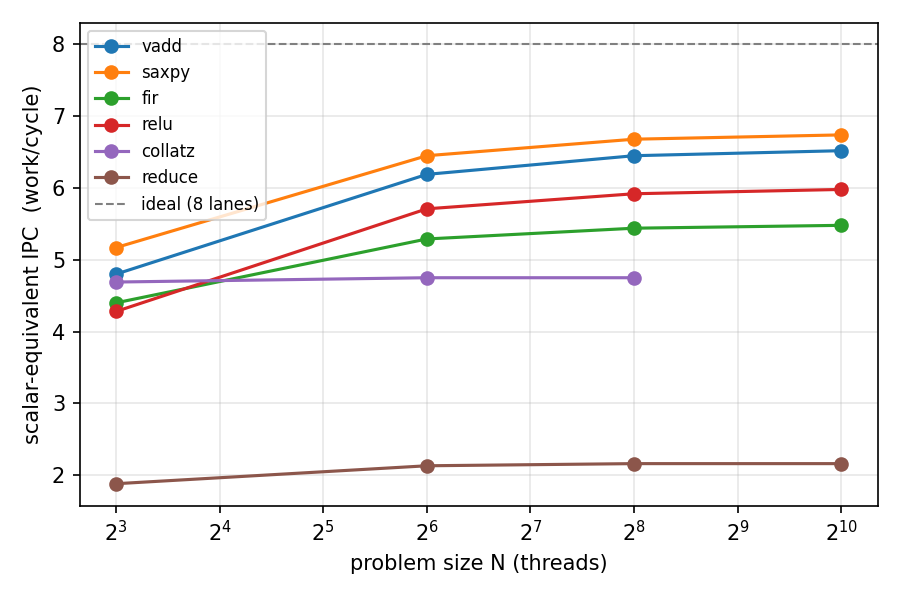
\includegraphics[width=0.8\textwidth]{throughput.png}
\caption{Scalar-equivalent throughput versus problem size. Throughput ramps as
occupancy rises (latency hiding) and saturates below the eight-lane ideal because
of the single shared data port.}
\label{fig:throughput}
\end{figure}

\begin{figure}[t]
\centering
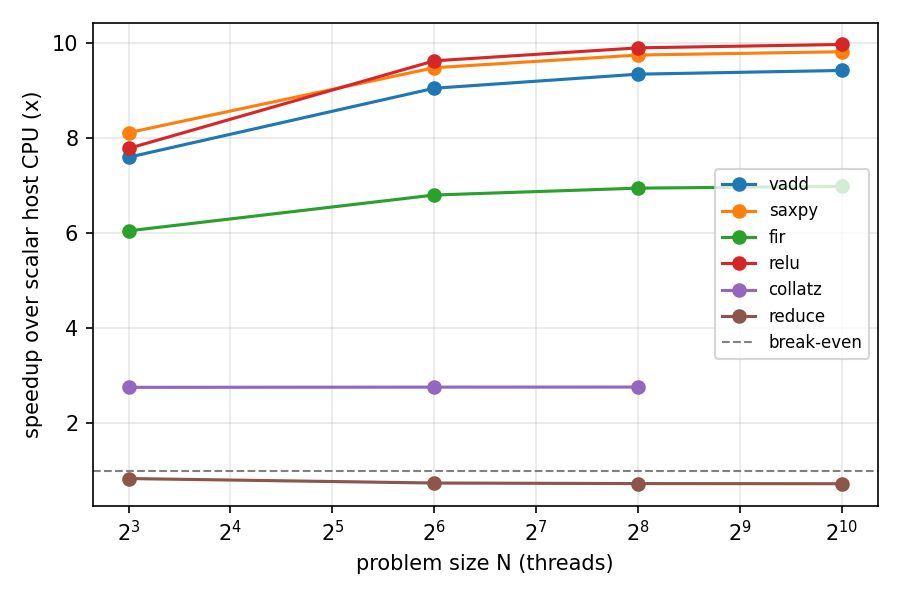
\includegraphics[width=0.8\textwidth]{speedup.png}
\caption{Measured speedup over the five-stage RV32I host running the same work.
Streaming kernels reach $7$--$10\times$; divergence reduces the gain; the serial
reduction falls below break-even.}
\label{fig:speedup}
\end{figure}

\section{Design-space exploration: lanes and warps}
\label{sec:dse}
Because the lane count and resident-warp count are elaboration parameters, all
twelve configurations of $\mathrm{NUM\_LANES}\in\{4,8,16,32\}$ against
$\mathrm{NUM\_WARPS}\in\{2,4,8\}$ were swept; all elaborate and pass the suite
bit-exact. Table~\ref{tab:dse} reports the geometric-mean throughput over the five
lane-count-agnostic kernels. Throughput scales almost linearly with lanes
($3.06\rightarrow5.85\rightarrow11.68\rightarrow23.24$ work-items/cycle, about
$1.97\times$ per doubling), and widening the lanes also widens the coalescing
line, so global traffic falls proportionally. The resident-warp count makes
essentially no difference here, because the behavioural memory model answers in a
single cycle and so offers almost no latency for extra warps to hide; the two
knobs are separable---lanes buy data-parallel throughput, warps buy latency
tolerance---and both cost register-file area.

\begin{table}[t]
\caption{Geometric-mean throughput (work-items/cycle) over the five lane-agnostic
kernels, swept over lanes and resident warps. All twelve configurations verify
bit-exact.}
\label{tab:dse}
\centering
\small
\begin{tabular}{lrrr}
\toprule
& \multicolumn{3}{c}{NUM\_WARPS}\\
\cmidrule(lr){2-4}
NUM\_LANES & 2 & 4 & 8\\
\midrule
4  & 3.06  & 3.06  & 3.05\\
8  & 5.85  & 5.85  & 5.85\\
16 & 11.68 & 11.68 & 11.65\\
32 & 23.24 & 23.24 & 23.14\\
\bottomrule
\end{tabular}
\end{table}

%------------------------------------------------------------------------------
\chapter{Floating-Point Extension}
\label{ch:fp}
%------------------------------------------------------------------------------

The base engine is integer-only. This chapter extends it with a per-lane
floating-point unit in both single (FP32) and half (FP16) precision, keeping the
same SIMT structure: the extension is a per-lane execute unit and a second
per-lane register file, not a new pipeline. It covers the full common arithmetic
set---add, subtract, multiply, the fused multiply-add, and division and square
root---plus the sign, compare, convert, and move operations, all in both
precisions. It matters to this thesis for two reasons: it establishes the timing
methodology later reused for the INT8 engine, and its rounding-correct FP path is
directly reused by the requantization step of Chapter~\ref{ch:requant}.

\section{The per-lane FP unit and register file}
Each lane gains a compact, fixed-latency floating-point unit beside its integer
ALU, and a second per-lane register file holds the 32 floating-point registers in
distributed RAM, addressed exactly like the integer VRF. The two files have
independent write ports, so an FP compute result and an integer load can retire in
the same cycle; only same-file collisions defer. Rounding is round-to-nearest-even,
float-to-integer truncates, and subnormals are flushed to zero---a deliberate
throughput-oriented choice that keeps each lane small.

\section{Half precision by widen--compute--narrow}
Half precision is not a second arithmetic datapath. A 16-bit half lives in a
32-bit register NaN-boxed (the upper 16 bits all ones), per the RISC-V convention.
For an FP16 operation the unit checks the box, widens the operand exactly to FP32,
runs the single-precision datapath, and rounds the FP32 result back to FP16. This
is correct, not approximate: because the FP32 intermediate carries a 24-bit
significand and $24\ge 2\cdot 11 + 2$, rounding first to FP32 and then to FP16
gives the same value as rounding directly to FP16, so FP16 add, subtract,
multiply, and the integer/FP16 conversions are correctly single-rounded. Half
precision thus reuses the verified single-precision logic almost entirely, adding
only the widen, narrow, and box steps---and, as shown below, at no extra cycle
cost.

\section{The fused multiply-add and the iterative SFU}
The fused multiply-add computes $\pm(a\cdot b)\pm c$ with a \emph{single}
rounding, so it cannot be built by chaining the multiplier and adder. The unit
forms the exact 48-bit product, anchors it in a wide fixed-point accumulator,
aligns the addend while capturing a sticky bit, and normalizes and rounds once.
Division and square root are produced one bit per cycle by a digit-recurrence and
are the engine's first multi-cycle operations. Because such a core is large, the
engine has a \emph{single shared} one rather than one per lane: when a warp issues
a divide or square root the engine captures all its lanes' operands, parks the
warp on a stall scoreboard, and sequences the active lanes through the shared core
one at a time---the same park-and-resume mechanism the memory engine uses, so the
scheduler keeps issuing other warps meanwhile.

\section{Verification}
Each unit is verified standalone against a DPI-C IEEE-754 reference: FP32 against
the host's correctly-rounded operations (including the fused \code{fmaf} and
\code{sqrtf}), and FP16 against an independent double-based reference. Over random
vectors spanning the product-dominant, balanced (cancellation), and
addend-dominant regimes, plus directed infinity, NaN, zero, flush-to-zero,
overflow, divide-by-zero, square-root-of-negative, mis-boxed-operand, and
conversion corners, the pipelined unit passes \num{96066} checks and the iterative
divide/square-root unit a further \num{20023}, all bit-exact
(Table~\ref{tab:fpverif})---\num{116089} checks with zero mismatches. End-to-end
kernels then run the complete warp pool bit-exact to 1024 threads.

\begin{table}[t]
\caption{Floating-point operation coverage. Every operation is implemented and
checked in both FP32 and FP16, bit-exact against an IEEE-754 reference.}
\label{tab:fpverif}
\centering
\small
\begin{tabular}{ll}
\toprule
Category & Operations (each in FP32 \emph{and} FP16)\\
\midrule
Arithmetic     & \code{fadd}, \code{fsub}, \code{fmul}\\
Fused          & \code{fmadd}, \code{fmsub}, \code{fnmsub}, \code{fnmadd}\\
Divide / root  & \code{fdiv}, \code{fsqrt} (iterative, multi-cycle)\\
Sign / select  & \code{fsgnj\{,n,x\}}, \code{fmin}, \code{fmax}\\
Compare        & \code{feq}, \code{flt}, \code{fle}\\
Convert        & float$\leftrightarrow$int, FP32$\leftrightarrow$FP16\\
Move / classify& \code{fmv.x.\_}, \code{fmv.\_.x}, \code{fclass}\\
\midrule
\multicolumn{2}{l}{Bit-exact checks vs.\ IEEE reference:
\textbf{\num{116089}} (0 mismatches)}\\
\bottomrule
\end{tabular}
\end{table}

\section{Area cost and the timing-closure study}
\label{sec:fppa}
Table~\ref{tab:fppa} gives the area cost: floating point raises LUTs from
\num{30088} to \num{74342} ($2.5\times$), flip-flops from \num{4590} to \num{7894},
and DSP blocks from 24 to 40, at \SI{1.34}{\watt}. The increase is dominated by
the common-case arithmetic unit---eight per-lane copies of the
add/multiply/FMA/convert datapath, the FMA being the largest single block---rather
than the iterative divide/square-root units, which synthesize to only \num{689}
LUTs each. As a single-cycle block the FMA's raw path is \SI{16.2}{\nano\second}
(\SI{61}{\mega\hertz}), making it the frequency bottleneck of the extension.

\begin{table}[t]
\caption{FP extension area cost: out-of-context synthesis of the accelerator on
\code{xczu7ev}, integer baseline versus FP-enabled.}
\label{tab:fppa}
\centering
\small
\begin{tabular}{lrrr}
\toprule
Resource & Integer & FP-enabled & $\Delta$\\
\midrule
LUTs         & \num{30088} & \num{74342} & $2.5\times$\\
\quad LUTRAM & \num{1428}  & \num{3348}  & --\\
Flip-flops   & \num{4590}  & \num{7894}  & $1.7\times$\\
DSP48E2      & 24          & 40          & $+16$\\
BRAM         & 0           & 0           & --\\
Power        & 0.81~W      & 1.34~W      & --\\
\bottomrule
\end{tabular}
\end{table}

The timing closure is a four-step, diagnosis-driven argument, summarised in
Table~\ref{tab:fpclose} and illustrated in Figure~\ref{fig:fpclosure}.

\paragraph{Step 1 --- two-stage FMA.} Pipelining the FP unit into two stages, split
at the FMA accumulator boundary, and absorbing the extra cycle in a single-slot
warp scoreboard, closes at \SI{78}{\mega\hertz}. The placed critical path is the
first FMA stage, but it is now \emph{routing}-dominated (7.4 of \SI{12.8}{\nano\second}
is wire delay): in the FP-enlarged fabric, interconnect, not logic depth, has
become the binding constraint.

\paragraph{Step 2 --- shared serial SFU.} Folding the eight per-lane
divide/square-root cores into one shared serial unit removes about \num{3700} LUTs
and \num{1200} flip-flops and drops power from \num{1.53} to \SI{1.22}{\watt}.
Crucially it leaves the FMA path structurally unchanged yet, by de-congesting the
fabric, cuts that path's routing delay and raises the placed maximum from 78 to
\SI{84.1}{\mega\hertz}---same logic, less congestion, higher frequency: a direct
confirmation that interconnect bounds the design.

\paragraph{Design-space check.} If congestion is the limit, does \emph{trimming}
the fabric help? Placing the FP design at four lanes halves its area (37k versus
69k LUTs, 20 versus 40 DSP) but reaches only \SI{79.7}{\mega\hertz}, marginally
\emph{below} the eight-lane \SI{84.1}{\mega\hertz}. The critical path is a
\emph{single} lane's FMA cone, whose logic depth is independent of the lane count;
the eight-lane configuration therefore Pareto-dominates the four-lane one (equal
frequency at twice the throughput) and the true frequency lever is the FMA
\emph{microarchitecture}, not the fabric size.

\paragraph{Step 3 --- three-stage FMA.} Acting on that finding, the FMA is split
across three stages---product, 128-bit align-and-add, and normalize-and-round---so
no single stage carries the whole cone. Place-and-route now \emph{meets} timing at
\SI{100.7}{\mega\hertz} (worst setup slack $+0.071$~ns), and decisively the
critical path moves \emph{off} the FMA onto the vector-register-file LUTRAM read
mux---the same structure that bounds the \emph{integer} design
(Section~\ref{sec:lutram}). The FP datapath is no longer the frequency limiter.

\paragraph{Deployable SoC.} Integrated into \code{chip\_top} with the host and the
eight-bank shared memory, and after splitting the scheduler's fetch/execute cloud
with a pipeline register, the full chip signs off with every port pin-constrained
for the ZCU104 and a warning-free design-rule check at $+0.360$~ns worst slack
(\SI{103.7}{\mega\hertz}), \num{71567} LUTs, \num{17834} flip-flops, 40 DSP, zero
BRAM, and \SI{1.20}{\watt}: a deployable bitstream, not only a timing report.

\begin{table}[t]
\caption{Placed post-route PPA of the FP-enabled accelerator across the
timing-closure steps and the lane design-space point (\code{xczu7ev},
out-of-context place-and-route unless noted, \SI{100}{\mega\hertz} constraint).
The three-stage FMA (step~3) is what meets \SI{100}{\mega\hertz}; the shared SFU
(step~2) and lane trimming help area and power but not the frequency floor. The
final row is the complete in-context SoC with ZCU104 pin constraints and a
warning-free DRC.}
\label{tab:fpclose}
\centering
\small
\setlength{\tabcolsep}{4pt}
\begin{tabular}{p{3.4cm}rrrrrrl}
\toprule
FP datapath & Lanes & LUT & FF & DSP & Power & Fmax & Crit.\ path\\
            &       &     &    &     & (W) & (MHz) & \\
\midrule
Two-stage FMA        & 8 & \num{72573} & \num{12347} & 40 & 1.53 & 78.0  & FMA cone\\
$+$ shared serial SFU& 8 & \num{68914} & \num{11153} & 40 & 1.22 & 84.1  & FMA cone\\
Three-stage FMA      & 8 & \num{69987} & \num{14954} & 40 & 1.22 & \textbf{100.7} & VRF LUTRAM\\
\emph{DSE:} four lanes & 4 & \num{36785} & \num{6953} & 20 & 0.98 & 79.7 & FMA cone\\
\emph{SoC:} deployable & 8 & \num{71567} & \num{17834} & 40 & 1.20 & \textbf{103.7} & FP ctl.\ broadcast\\
\bottomrule
\end{tabular}
\end{table}

\begin{figure}[t]
\centering
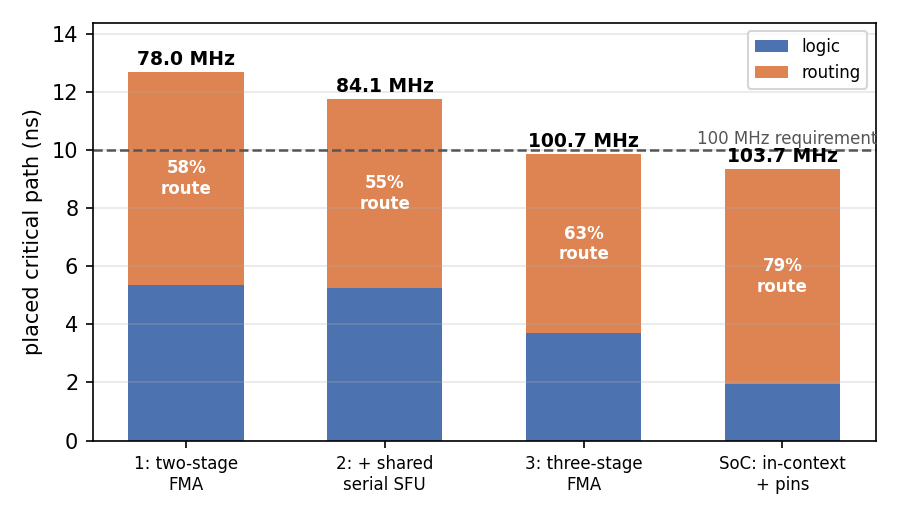
\includegraphics[width=0.8\textwidth]{fp_closure.png}
\caption{Placed critical path at each closure step, split into logic and routing
delay. Every step is routing-dominated; the three-stage FMA closes timing by
shortening the whole cone, not by reducing the wire share.}
\label{fig:fpclosure}
\end{figure}

\section{Floating-point throughput}
On streaming kernels the added pipeline latency is fully hidden by SIMT warp
interleaving; the FP16 points lie exactly on the FP32 curves and the cycle counts
are identical, because half precision shares the same pipelined datapath. Half
precision therefore delivers reduced storage and bandwidth at \emph{no} throughput
penalty. Table~\ref{tab:fpkernels} reports four toolchain-assembled FP application
kernels, each verified bit-exact. Two effects stand out: the iterative
divide/square-root unit makes \code{fnorm} about $6\times$ the cycles of the
streaming \code{fsaxpy}, the honest price of correctly-rounded transcendental
support on a small iterative core; and \code{fdot}'s single-lane reduction runs at
\SI{45}{\percent} lane utilization, so by Eq.~\eqref{eq:energy} the idle
\SI{55}{\percent} is lane-datapath energy a mask-gated design clocks away---an
amount that grows because the FP unit makes each lane substantially larger.

\begin{table}[t]
\caption{FP application kernels (FP32 unless noted), verified bit-exact. Cycles,
global line transactions, and lane utilization at $N{=}256$.}
\label{tab:fpkernels}
\centering
\small
\begin{tabular}{llrrr}
\toprule
Kernel & Computation & Cycles & Gmem & Lane-util\\
\midrule
\code{fsaxpy}   & $\alpha A_i + B_i$ (fmadd)  & 419      & 96 & 100\%\\
\code{fsaxpy16} & $\alpha A_i + B_i$ (FP16)   & 451      & 96 & 100\%\\
\code{fnorm}    & $A_i/\sqrt{B_i}$ (div+sqrt) & \num{2396} & 96 & 100\%\\
\code{fdot}     & $\sum_l A_{8w+l}B_{8w+l}$   & \num{1991} & 96 & 45\%\\
\bottomrule
\end{tabular}
\end{table}

%------------------------------------------------------------------------------
\chapter{The \texttt{pdot8} INT8 Dot-Product Instruction}
\label{ch:pdot8}
%------------------------------------------------------------------------------

This chapter begins the transformation of SIMTiX into an AI inference
accelerator. The gap between ``can run neural-net math'' and ``is an efficient
inference accelerator'' is arithmetic precision and density. A general SIMT core
\emph{can} do INT8 by masking and shifting bytes, but that costs about eight
instructions per four multiply-accumulates (MACs). A single fused dot-product
instruction collapses that to one instruction and maps the four multiplies onto
the FPGA's hard DSP48E2 blocks. \code{pdot8} is that instruction.

\section{Rationale}
A prior resource audit established that SIMTiX uses only about \SI{2.3}{\percent}
of the device DSP blocks and no BRAM: the FPGA has enormous arithmetic headroom.
\code{pdot8} spends a little of that DSP headroom---four blocks per lane---to buy a
$4\times$ INT8 throughput multiplier, exactly the right trade for a design that is
nowhere near DSP-bound. Three design decisions define the instruction.

\paragraph{Non-accumulating semantics.} \code{pdot8 rd, rs1, rs2} computes a pure
four-way dot product into \code{rd}; it does not read \code{rd} as a running
accumulator. The integer register file has exactly two asynchronous read ports; a
fused \code{rd += dot} would need a third read port on every lane's bank. The
non-accumulating form keeps the two-port file untouched, and the kernel
accumulates in a separate register with a single-cycle \code{add} that overlaps
the next \code{pdot8} under the scheduler.

\paragraph{A background DSP engine, not a single-cycle ALU op.} \code{pdot8}
executes in a park-and-resume background engine (\code{W\_DOT}), exactly like the
RV32M \code{mul} engine and the FP compute engine, not in the single-cycle ALU.
Putting a DSP multiply directly in the single-cycle fetch$\rightarrow$execute
cloud is precisely what hurt timing historically; a pipelined, parked DSP stays
off the critical path, and the scheduler keeps issuing other warps while the DSP
tree fills.

\paragraph{Custom-0 opcode, encoded with \code{.insn}.} \code{pdot8} uses the
RISC-V custom-0 major opcode, which the ISA reserves for non-standard extensions,
so it can never collide with the instructions the toolchain emits and is inert to
every existing kernel and to the compiler. Because gcc does not know the mnemonic,
kernels encode it with the assembler's raw \code{.insn r} directive---no compiler
patch is needed.

\section{Instruction specification}
\code{pdot8} is an R-type instruction under the custom-0 opcode. For
$\code{rs1}=\{a_3,a_2,a_1,a_0\}$ and $\code{rs2}=\{b_3,b_2,b_1,b_0\}$, where byte
$i$ occupies bits $[8i+7:8i]$,
\begin{equation}
\code{rd} = \sum_{i=0}^{3}\mathrm{ext}(a_i)\times\mathrm{ext}(b_i),
\end{equation}
where $\mathrm{ext}(\cdot)$ is sign-extension for a signed operand and
zero-extension for an unsigned one, selected by \code{funct3}
(Table~\ref{tab:pdot8}). The sum of four products lies within
$[-260100,+260100]$, so it never overflows the 32-bit destination. A single signed
$9\times 9$ multiply serves every variant, because an unsigned byte extended with a
zero sign bit is non-negative and a signed byte is sign-extended.

\begin{table}[t]
\caption{The \code{pdot8} signedness variants (\code{funct3}). The signed$\times$
unsigned form is the weight$\times$activation case of inference.}
\label{tab:pdot8}
\centering
\small
\begin{tabular}{llll}
\toprule
\code{funct3} & Mnemonic & \code{rs1}$\times$\code{rs2} & Typical use\\
\midrule
\code{000} & \code{pdot8}   & signed $\times$ signed   & symmetric / weight$\times$weight\\
\code{001} & \code{pdot8u}  & unsigned $\times$ unsigned & activation$\times$activation\\
\code{010} & \code{pdot8su} & signed $\times$ unsigned  & weight $\times$ activation (inference)\\
\bottomrule
\end{tabular}
\end{table}

\section{Microarchitecture}
\code{pdot8} is a faithful clone of the integer-multiply engine. Operands are
captured at issue and held constant while the warp is parked, so the datapath is a
fixed-latency streaming pipeline. Per lane, the four byte-pairs are extended to
9-bit signed values (the DSP A/B registers), four signed $9\times 9$ products are
formed (the DSP MREG), registered (the DSP PREG), and reduced by a registered
adder tree. From issue to a settled result is six cycles: operand capture, A/B
register, multiply, product register, and two adder stages. A three-state
scoreboard (\code{DOT\_IDLE}$\rightarrow$\code{DOT\_RUN}$\rightarrow$\code{DOT\_WB})
captures the result one safe cycle after it settles and drives it onto the integer
register file when the port is free, then restores the parked warp's PC. Only one
dot is in flight across all warps; a second warp attempting a dot simply waits and
retries, which is safe because nothing was committed. Listing~\ref{lst:pdot8}
shows the resulting inner loop.

\begin{lstlisting}[caption={INT8 dot-product inner loop: one \code{pdot8} per four
MACs, versus four multiplies and four adds plus byte extraction for a scalar
equivalent.},label={lst:pdot8}]
.Lk:  lw   av, 0(pa)                 # 4 activations (packed int8)
      lw   wv, 0(pw)                 # 4 weights     (packed int8)
      .insn r 0x0B, 2, 0, t0, wv, av # pdot8su t0 = sum_i w_i*a_i  (4 MACs)
      add  acc, acc, t0              # accumulate (single-cycle, overlaps)
      addi pa, pa, 4
      addi pw, pw, 4
      addi k,  k,  -4
      bnez k, .Lk
\end{lstlisting}

\section{Verification and cost}
The instruction is verified bit-exact: a single warp of eight lanes computes all
three variants on distinct operands, including the signed edge values $-128$, $127$
and $-1/255$ so sign and zero extension are exercised at the boundaries, and every
lane's result is checked against an exact integer reference---all eight lanes and
three variants pass. Because the arithmetic is integer, the reference has no
tolerance. Table~\ref{tab:ai_ppa} gives the measured FPGA cost, placed
out-of-context on the \code{xczu7ev} against the FP-enabled M17 baseline: the INT8
engine adds \num{32} DSP blocks (four per lane across eight lanes) and about
\SI{1}{\percent} of the LUTs, and---crucially---does \emph{not} regress the
operating frequency, because it is a pipelined DSP background engine off the
fetch$\rightarrow$execute path. This is the central design claim of the INT8
extension, confirmed by measurement.

\begin{table}[t]
\caption{Measured FPGA PPA of the INT8-enabled accelerator (FP $+$ \code{pdot8}),
placed out-of-context on \code{xczu7ev} at a \SI{100}{\mega\hertz} constraint,
versus the FP-only baseline.}
\label{tab:ai_ppa}
\centering
\small
\begin{tabular}{lrrr}
\toprule
Resource & FP $+$ \code{pdot8} & FP baseline & $\Delta$\\
\midrule
LUT          & \num{70779} (30.7\%) & \num{69987} & $+792$ ($\sim$1\%)\\
Flip-flops   & \num{17411}          & \num{14954} & $+2457$\\
DSP48E2      & \textbf{72} (4.2\%)  & 40          & $\mathbf{+32}$\\
BRAM         & 0                    & 0           & 0\\
Placed Fmax  & \textbf{112.2}~MHz   & 100.7~MHz   & $+11.5$\\
Power        & 0.969~W              & 1.22~W      & --\\
\bottomrule
\end{tabular}
\end{table}

%------------------------------------------------------------------------------
\chapter{Quantized GEMM and GEMV Kernels}
\label{ch:gemm}
%------------------------------------------------------------------------------

GEMM (general matrix multiply) is the computational core of every neural-network
layer---fully-connected layers \emph{are} GEMMs, and convolution becomes a GEMM
after \code{im2col}---so a correct, coalesced INT8 GEMM is the load-bearing kernel
of the inference story. This chapter builds two kernels on \code{pdot8}: a GEMM
tile (\code{qgemm}) and, for the MLP layers, a GEMV (\code{qgemv}).

\section{The INT8 GEMM tile}
\code{qgemm} computes a full $8\times 8$ output tile with reduction length $K=16$:
$C[r][c]=\sum_{k=0}^{K-1}A[r][k]\cdot B[k][c]$, with signed INT8 operands and an
INT32 accumulator. One warp maps to each output row and one lane to each output
column, so all eight lanes of a warp share the same row of $A$ and each lane owns a
different column of $B$ and $C$. The reduction runs four elements at a time with
\code{pdot8}.

The data layouts are the crux, chosen so that both operand loads coalesce
(Table~\ref{tab:layouts}). $A$ is stored row-major, so all eight lanes of a warp
read the \emph{same} address---a single broadcast line transaction. $B$ is stored
\emph{pre-packed} as $\mathit{Bpacked}[K/4][N]$, so that for a fixed reduction group
the eight columns are contiguous---a single coalesced line. This is the standard
inference weight layout: weights are packed offline. The little-endian byte packing
matches \code{pdot8}'s operand format exactly.

\begin{table}[t]
\caption{\code{qgemm} data layouts, chosen so both operand loads coalesce to a
single line transaction.}
\label{tab:layouts}
\centering
\small
\begin{tabular}{p{1.1cm}p{5.2cm}p{5.0cm}}
\toprule
Matrix & Layout & Why it coalesces\\
\midrule
$A$ & $8\times16$ INT8, row-major & every lane of a warp uses the same row
$\Rightarrow$ one broadcast line\\
$B$ & pre-packed $\mathit{Bpacked}[4][8]$ words & the eight columns of a group are
contiguous $\Rightarrow$ one coalesced line\\
$C$ & $8\times8$ INT32, row-major & the eight columns of a row are contiguous
$\Rightarrow$ one store line per warp\\
\bottomrule
\end{tabular}
\end{table}

\section{Performance}
Table~\ref{tab:qgemm} gives the measured performance. The kernel does $1024$ MACs
in $538$ cycles, a throughput of $1.90$ MAC/cycle against a datapath ceiling of
$32$ (eight lanes $\times$ four MACs). The \num{72} global-memory transactions
match the analytic coalescing model exactly---$8\ \text{warps}\times(K/4\ \text{loads}
\times 2 + 1\ \text{store})=8\times 9$---an $8\times$ reduction versus the $576$ of a
naive per-lane engine, which confirms that coalescing works as designed. The
throughput is functional rather than tuned: the gap to the ceiling is two honest
and known limits---the single-slot \code{W\_DOT} scoreboard (only one \code{pdot8}
in flight, its latency only partly hidden by eight warps of work), and the
per-warp \code{load}$\rightarrow$\code{pdot8}$\rightarrow$\code{accumulate}
dependency chain. The lever for real density is not more SIMT tuning but a
tensor/systolic engine, for which \code{qgemm} establishes the correct, coalesced
baseline.

\begin{table}[t]
\caption{Measured performance of the \code{qgemm} INT8 GEMM tile ($M{=}N{=}8$,
$K{=}16$).}
\label{tab:qgemm}
\centering
\small
\begin{tabular}{lrl}
\toprule
Metric & Value & Notes\\
\midrule
MACs & \num{1024} & $M\cdot N\cdot K = 8\cdot 8\cdot 16$\\
\code{pdot8} SIMT instructions & 32 & $M\cdot(K/4)$; each spans $N$ lanes $\times 4$\\
Cycles & 538 & measured\\
Throughput & $1.90$ MAC/cycle & ceiling $= 32$ (8 lanes $\times$ 4)\\
Global-mem transactions & 72 & $= 8\ \text{warps}\times(K/4\cdot 2 + 1)$\\
\bottomrule
\end{tabular}
\end{table}

At the measured placed power of \SI{0.969}{\watt}, and counting operations as
twice the MAC rate, the measured efficiency is $0.39$~GOP/s/W and the datapath
ceiling is $6.6$~GOP/s/W at \SI{100}{\mega\hertz}. For an eight-lane academic core
these land honestly in the GOPS range, not TOPS; the measured-to-ceiling gap is
the motivation for a future tensor engine.

\section{The GEMV layer primitive}
A fully-connected MLP layer with a single input vector is a matrix--vector product
(GEMV), not a full GEMM. \code{qgemv} computes $\mathit{out}[n]=\sum_{k}x[k]\cdot
W[k][n]$ with one lane per output element $n$, reducing $K$ four at a time with
\code{pdot8}. It is parameterized so the \emph{same} kernel runs both MLP layers:
the reduction length is read as $K/4$ from a configuration word at a fixed address,
and the number of outputs $N$ (the weight-column stride) is the seeded thread
count. The input vector $x$ is broadcast (shared by all lanes) and the weights are
the same pre-packed $\mathit{Wpacked}[K/4][N]$ layout as \code{qgemm}, so both
loads coalesce. Listing~\ref{lst:qgemv} shows the kernel; it is the primitive the
MNIST engine of Chapter~\ref{ch:mnist} launches, once per layer.

\begin{lstlisting}[caption={The parameterized INT8 GEMV kernel. \code{Kp} is read
from a config word; \code{N} is the seeded thread count \code{a4}. The K-loop is
uniform, so it never diverges.},label={lst:qgemv}]
_start:
    li      t0, 0x100          # config address
    lw      t1, 0(t0)          # t1 = Kp = K/4
    slli    t2, a0, 2          # &Wpacked[0][n] = a2 + n*4
    add     t2, a2, t2
    slli    t3, a4, 2          # N*4 = W column stride (bytes) per kk
    mv      t4, a1             # &x[0]
    li      t5, 0              # acc = 0
    li      t6, 0              # kk  = 0
.Lk:
    lw      s0, 0(t4)          # x[4kk..]           (broadcast)
    lw      s1, 0(t2)          # W[4kk..][n]        (coalesced)
    .insn r 0x0B, 0, 0, s2, s0, s1   # pdot8 (4 MACs)
    add     t5, t5, s2         # acc += partial dot
    addi    t4, t4, 4          # x += 1 word
    add     t2, t2, t3         # W += N words
    addi    t6, t6, 1
    blt     t6, t1, .Lk        # uniform loop
    slli    s3, a0, 2          # out[n] = acc
    add     s3, a3, s3
    sw      t5, 0(s3)
    ecall
\end{lstlisting}

%------------------------------------------------------------------------------
\chapter{Requantization}
\label{ch:requant}
%------------------------------------------------------------------------------

Requantization is the bridge that lets quantized layers be chained. A quantized
layer multiplies INT8 activations by INT8 weights into an INT32 accumulator---which
is exactly what \code{qgemm} and \code{qgemv} produce---but the next INT8 layer
needs INT8 \emph{inputs}. Requantization rescales the wide accumulator back to a
signed byte, per Eq.~\eqref{eq:requant}. Without it, the layers cannot compose.

\section{FP-reuse, not a dedicated datapath}
Because SIMTiX already has a full FP32 pipeline (Chapter~\ref{ch:fp}),
requantization is a short branchless FP sequence and needs \emph{no new hardware}.
This is a deliberate, honest trade. A production FPU-less INT8 accelerator would
implement requantize as a fixed-point integer datapath specifically to avoid
paying for an FPU; SIMTiX already pays for one, so the marginal-cost-optimal choice
is to reuse it. The kernel (Listing~\ref{lst:requant}) runs one thread per element:
it converts the accumulator to FP32, computes $\mathit{acc}\cdot\mathit{scale}+\mathit{zp}$
with a single fused rounding, clamps in floating point with branchless
\code{fmin}/\code{fmax} (so there is no SIMT divergence), rounds to nearest even on
the float-to-integer conversion, and stores a signed byte at stride one. Because
consecutive lanes' bytes pack into one word, the output is already in the next
layer's packed-INT8 input layout, with no repacking.

\begin{lstlisting}[caption={The requantization kernel (FP-reuse). The clamp is done
in floating point, before the integer conversion, so it is branchless and does not
diverge. A \emph{requant\_relu} variant clamps the low bound to 0 to fuse the ReLU
activation.},label={lst:requant}]
_start:                       # a0=tid a1=&Acc(int32) a2=&params(f32) a3=&Out(int8)
    slli     t0, a0, 2
    add      t1, a1, t0
    lw       t2, 0(t1)        # acc (int32)
    flw      f1, 0(a2)        # scale
    flw      f2, 4(a2)        # zero_point
    fcvt.s.w f3, t2           # (float)acc
    fmadd.s  f3, f3, f1, f2   # acc*scale + zp   (fused -> single rounding)
    lui  t3,0x42fe0; fmv.w.x f4,t3   #  127.0f
    lui  t3,0xc3000; fmv.w.x f5,t3   # -128.0f
    fmin.s   f3, f3, f4       # clamp high
    fmax.s   f3, f3, f5       # clamp low
    fcvt.w.s t4, f3, rne      # round to nearest even -> [-128,127]
    add      t5, a3, a0
    sb       t4, 0(t5)        # signed byte (packs 4/word)
    ecall
\end{lstlisting}

For the MLP an activation-fused variant, \emph{requant\_relu}, clamps the low bound
to $0$ instead of $-128$, performing the requantization and the ReLU activation in
a single pass---precisely what is needed between two fully-connected layers.

\section{Precision and verification}
The int-to-float conversion is exact for accumulators below $2^{24}$; for the MNIST
MLP ($784$ inputs, $|\mathit{acc}|\lesssim 1.3\times 10^{7}<2^{24}$) the accumulator
is within the exact range, so no precision is lost in the conversion. The kernel is
verified bit-exact: eight accumulators spanning the sign range, both clamp
saturations, and the boundary values are checked against a software reference, and
all eight requantized bytes match. A verification aside worth recording: the first
run appeared to fail, but the \emph{reference} was wrong---SystemVerilog's
\code{int'(real)} cast already rounds to nearest, and the reference had additionally
added $0.5$, double-rounding one value; the hardware was correct. A golden model is
only as trustworthy as its own arithmetic.

%------------------------------------------------------------------------------
\chapter{End-to-End On-Chip MNIST Inference}
\label{ch:mnist}
%------------------------------------------------------------------------------

This is the capstone. A trained, quantized $784{\rightarrow}128{\rightarrow}10$
multilayer perceptron classifies MNIST handwritten digits, and the entire forward
pass runs end-to-end on the integrated chip: the host CPU streams the weights out
of an on-chip block-RAM store into the accelerator's working memory in tiles,
launches the kernels of the previous chapters over the memory-mapped interface, and
reads back the predicted digit. It is the proof point that SIMTiX is not a core that
merely \emph{can} do neural-network math, but one that runs a real, trained,
quantized network end-to-end and gets the right answers.

\section{The model and its quantization}
A $784{\rightarrow}128{\rightarrow}10$ ReLU MLP was trained in pure numpy (SGD,
eight epochs), reaching \SI{96.82}{\percent} FP32 test accuracy. It was then
quantized with symmetric per-tensor INT8: activations and weights scaled to
$[-127,127]$. The INT8 test accuracy is \SI{96.53}{\percent}---a drop of only
\SI{0.29}{\percent}, confirming that INT8 is essentially free in accuracy for this
network. The layer-1 requantization multiplier is
$M_1=(S_x\,S_{w1})/S_h=0.000696921$. A crucial detail for bit-exact verification:
the golden reference computes the requantization in \emph{float32}, matching the
hardware FPU exactly rather than in float64, so the hardware can be held to a
digit-for-digit standard. The model script exports the weights, the test images,
and the integer-exact golden predictions as packed hex.

\section{Per-image inference dataflow}
Each $28\times 28$ image is flattened to a 784-vector, quantized to INT8, and run
through the network. The forward pass is
\[
x(\mathrm{int8}[784])\ \xrightarrow{\ \code{qgemv}\ }\ \mathit{acc_1}(\mathrm{int32}[128])
\ \xrightarrow{\ \code{requant\_relu}\ }\ h(\mathrm{int8}[128])
\ \xrightarrow{\ \code{qgemv}\ }\ \mathit{acc_2}(\mathrm{int32}[10])
\ \xrightarrow{\ \mathrm{argmax}\ }\ \text{digit}.
\]
The same \code{qgemv} runs both layers: for layer~1 the configuration word holds
$K/4=196$ and the launch requests $N=128$ outputs; for layer~2 it holds $K/4=32$
and $N=10$. The layouts are chosen so each stage's output is already the next
stage's input format: \code{requant\_relu} stores the 128 hidden bytes packed four
per word, exactly \code{qgemv}'s packed input-vector layout for layer~2, with no
repacking.

\section{The on-chip integration challenge}
\label{sec:onchip}
Running this on the real chip, rather than in a testbench that owns a large flat
memory, poses a concrete architectural problem. The accelerator reads its operands
from the on-chip shared memory, which is distributed-RAM (LUTRAM) and was enlarged
to 16~KB for this demonstration. But the first weight matrix alone,
$W_1\in\mathbb{Z}^{196\times 128}$ packed, is \num{25088} 32-bit words---about
98~KB---which does not fit. Placing the full weight set in LUTRAM would cost tens of
thousands of LUTs and is impractical. Moreover, the entire chip, host and
accelerator alike, assumes an asynchronous single-cycle memory, whereas block RAM
is synchronous with a one-cycle read latency; putting BRAM directly in the
accelerator's combinational load path would require risky surgery on the memory
engine and would break timing closure.

The chosen architecture leaves the accelerator core \emph{untouched}. The weights
live in a dedicated block-RAM store that only the host CPU reads; the CPU
\emph{streams} them, in tiles, into the accelerator's asynchronous LUTRAM working
memory. This is exactly the weights-in-BRAM, tile-into-fabric motif that real
inference accelerators use. The host CPU already honours a memory-ready handshake
(its pipeline stalls while the ready signal is low), so the block RAM's one-cycle
latency is absorbed by a single-cycle CPU stall on each weight read, added in the
chip's top level. Table~\ref{tab:chipmap} shows the resulting chip address map: a
new region routes to the block-RAM weight store, another to the accelerator's MMIO
page, another to the result register, and the remainder to the working memory.

\begin{table}[t]
\caption{Chip address map for the on-chip MNIST configuration. The block-RAM
weight store is a new region ($\mathtt{0xA}$); the host CPU stalls one cycle on
each weight read to absorb the synchronous-BRAM latency.}
\label{tab:chipmap}
\centering
\small
\begin{tabular}{lll}
\toprule
Region (top nibble) & Target & Access\\
\midrule
\code{0x9} & chip result register & write: latch result, raise \code{done}\\
\code{0x8} & accelerator MMIO page & command / status\\
\code{0xA} & block-RAM weight store & read-only, 1-cycle stall\\
else       & 16~KB LUTRAM working memory & asynchronous, single-cycle\\
\bottomrule
\end{tabular}
\end{table}

\section{The host driver}
The host driver is a \num{182}-instruction RV32I program, assembled to an
instruction ROM. It performs the entire inference under the memory-mapped
interface, with no custom host instructions. Because the working memory cannot hold
$W_1$ at once, the driver \emph{tiles} the first layer: for each tile of 16 output
columns (eight tiles cover the 128 outputs) it copies that tile's weights out of
the block-RAM store into the working memory, repacked to the tile's column stride,
and launches \code{qgemv} on the tile; the second layer's weights are small enough
to stream in a single tile. The driver's structure per image is:
\begin{enumerate}
\item copy the image's 196 packed words into the working memory;
\item for each of the eight column-tiles of layer~1: stream the tile's weights
($196\times 16$ words, repacked so the kernel reads them at stride 16) from the
block-RAM store into the working memory, then launch \code{qgemv} with $N=16$ and
the output base offset to that tile;
\item launch \code{requant\_relu} over the 128 accumulators to produce the hidden
activations;
\item stream $W_2$ and launch \code{qgemv} with $N=10$ for layer~2;
\item argmax the ten logits (a signed integer scan) to obtain the predicted digit,
and self-check it against the on-chip golden.
\end{enumerate}
After all 64 images the driver publishes the count of golden-matching predictions
to the result register. Two engineering details were essential. First, a
\emph{two-phase} kernel-completion poll: the dispatcher parks in its done state
with \code{DONE} held high after each kernel, so a naive poll would immediately
observe the \emph{previous} kernel's stale \code{DONE}; the driver instead waits
first for \code{BUSY} to assert and only then for \code{DONE}, which is robust
across the roughly 640 kernel launches of the full run. Second, the repacking
arithmetic must place tile weights so that the kernel, told a column stride of 16,
reads exactly $W_1[kk][n_0+n]$---verified against the kernel's addressing before
simulation.

\section{Result}
The design was simulated at the full chip level. The chip boots, the host CPU
drives the whole inference, and the result is unambiguous:
\begin{center}
\emph{golden-match count $=64/64$; completed in ${\sim}10.7$ million cycles.}
\end{center}
The chip reproduces the integer-exact software golden for \emph{all 64 test
images, bit-for-bit}. Table~\ref{tab:mnist} summarises the model and the result.
The chip's predictions match the true image labels on 63 of the 64 images
(\SI{98.4}{\percent}); the single miss is a genuine model misclassification---a
sloppily written digit `5' read as `6', not a hardware error, since every one of
the 64 outputs is bit-identical to the software golden.
Figure~\ref{fig:montage} shows the 64 images the chip classifies, each labelled
with the chip's prediction and the true label.

\begin{table}[t]
\caption{The quantized MNIST MLP and its end-to-end on-chip result.}
\label{tab:mnist}
\centering
\small
\begin{tabular}{ll}
\toprule
Quantity & Value\\
\midrule
Network & $784\rightarrow128\rightarrow10$ MLP, ReLU\\
FP32 test accuracy & 96.82\%\\
INT8 test accuracy & 96.53\% ($-0.29\%$)\\
Layer-1 requant multiplier $M_1$ & 0.000696921\\
On-chip result vs.\ golden & \textbf{64 / 64 bit-exact}\\
On-chip accuracy vs.\ labels & 63 / 64 $=$ 98.4\%\\
Full-run latency & ${\sim}10.7$M cycles (64 images)\\
Weight store & 256~KB block RAM (host-streamed)\\
\bottomrule
\end{tabular}
\end{table}

\begin{figure}[t]
\centering
\includegraphics[width=0.86\textwidth]{mnist_montage.png}
\caption{The 64 MNIST test images classified end-to-end on the chip. Each tile
shows the exact INT8 pixels the accelerator processes, labelled with the chip's
prediction \emph{p} and the true label \emph{t}. The single red label is the one
genuine model misclassification (a `5' read as `6'); all 64 chip outputs are
bit-identical to the software golden.}
\label{fig:montage}
\end{figure}

The existing integer bring-up demonstration (the ``result $=964$'' checksum) shares
the same top-level and continues to pass unchanged, so the MNIST configuration is a
clean, parameter-selected mode of the same chip rather than a fork. This completes
the arc from a general SIMT core to a demonstrated, on-chip, end-to-end quantized
inference engine.

%------------------------------------------------------------------------------
\chapter{Consolidated Results and Discussion}
\label{ch:results}
%------------------------------------------------------------------------------

This chapter draws the measured results together and reads them as one story.

\section{Area and frequency across the design's evolution}
Table~\ref{tab:evolution} traces the accelerator through its three major
incarnations on the same device. The integer baseline, after the distributed-RAM
register file, is a \num{30088}-LUT, \num{24}-DSP design that meets
\SI{100}{\mega\hertz}. The floating-point extension multiplies the LUTs by
$2.5\times$ and, through the three-stage FMA closure, still meets
\SI{100}{\mega\hertz} with the critical path moved onto the register-file read
mux. The INT8 extension then adds \num{32} DSP blocks and about \SI{1}{\percent}
of the LUTs on top of the FP design without regressing frequency
(\SI{112.2}{\mega\hertz} placed). The consistent thread is that the arithmetic
extensions are cheap in LUTs and are kept off the critical path; the binding
constraint throughout is the register-file read multiplexer and interconnect
congestion, not the compute.

\begin{table}[t]
\caption{The accelerator across its three incarnations (placed out-of-context on
\code{xczu7ev}). Each extension is deliberately kept off the frequency-limiting
path.}
\label{tab:evolution}
\centering
\small
\begin{tabular}{lrrrr}
\toprule
Configuration & LUT & FF & DSP & Placed Fmax\\
\midrule
Integer (LUTRAM VRF)      & \num{30088} & \num{4590}  & 24 & $\ge$100~MHz\\
$+$ Floating point (3-stage FMA) & \num{69987} & \num{14954} & 40 & 100.7~MHz\\
$+$ INT8 \code{pdot8}     & \num{70779} & \num{17411} & 72 & 112.2~MHz\\
\bottomrule
\end{tabular}
\end{table}

\section{Reading each result}
\paragraph{The LUTRAM result (Table~\ref{tab:ppa_base}).} The $5.7\times$ LUT
reduction is the enabling result of the whole thesis: it is what makes a
readable SIMT design also a \emph{fittable} one, and it identifies the register
file, not the ALUs, as the true cost centre---a lesson that recurs at every later
stage, where the register-file read mux keeps re-emerging as the critical path.

\paragraph{The benchmark speedups (Table~\ref{tab:speedup}).} The $7$--$10\times$
on streaming kernels, $2.76\times$ under heavy divergence, and $0.72\times$ on the
serial reduction together map the SIMT model's operating envelope honestly. The
sub-unity reduction is not hidden; it says precisely that a reduction needs a
dedicated hardware primitive, and it is consistent with the \SI{39.8}{\percent}
lane utilization that Eq.~\eqref{eq:energy} converts into a large clock-gating
opportunity.

\paragraph{The FP verification and closure (Tables~\ref{tab:fpverif},
\ref{tab:fpclose}).} The \num{116089} bit-exact checks establish IEEE-754
correctness including the fused multiply-add and iterative divide/square root in
both precisions. The closure table is a diagnosis in five rows: the two-stage FMA
exposes a routing-bound path, the shared SFU confirms congestion by \emph{raising}
frequency with unchanged logic, the four-lane point rules out fabric size as the
lever, and the three-stage FMA closes \SI{100}{\mega\hertz} by shortening the cone
itself---after which the deployable SoC signs off at \SI{103.7}{\mega\hertz}.

\paragraph{The INT8 cost (Table~\ref{tab:ai_ppa}).} The design claim---INT8
throughput for \num{32} DSP and \SI{1}{\percent} LUT, with no frequency
regression---is confirmed by measurement, and it is confirmed \emph{because} the
engine is a pipelined DSP kept off the fetch$\rightarrow$execute path.

\paragraph{The GEMM throughput (Table~\ref{tab:qgemm}).} The $8\times$
memory-traffic reduction matches the analytic coalescing model exactly, validating
the layout design; the $1.90$-of-$32$ MAC/cycle throughput is reported with its two
known causes and its clear next lever (a tensor engine).

\paragraph{The MNIST result (Table~\ref{tab:mnist}).} The $64/64$ bit-exact
on-chip result is the thesis's proof point: a real, trained, quantized network runs
end-to-end through the integrated chip and matches the software golden digit for
digit, with the weights streamed from block RAM exactly as a deployable inference
accelerator would.

\section{Limitations and honest boundaries}
Several results are deliberately reported as limits rather than smoothed over. The
single shared data port caps SIMT throughput below the lane-count ideal. The serial
reduction is slower than the scalar host. The \code{qgemm} throughput is far below
its datapath ceiling because of the single-slot dot engine and the per-warp
dependency chain. The lane clock-gating saving is an analytic model from hardware
counters, not a gate-level power measurement. And the block-RAM-inclusive PPA of
the MNIST chip configuration---as opposed to the accelerator-only INT8 PPA of
Table~\ref{tab:ai_ppa}---is the one measurement not yet taken; it is the immediate
next step, and it is expected to show the first non-zero block-RAM usage in the
design (roughly 57 block-RAM tiles for the 256~KB weight store). Reporting these
boundaries is part of the contribution: the evaluation is a map of where the design
does and does not pay, not a highlight reel.

%------------------------------------------------------------------------------
\chapter{Conclusion and Future Work}
\label{ch:conclusion}
%------------------------------------------------------------------------------

\section{Conclusion}
This thesis has presented SIMTiX, a compact, fully-open RISC-V SIMT accelerator,
and carried it from a general-purpose parallel core to a demonstrated, on-chip,
end-to-end quantized neural-network inference engine. The baseline design fits the
complete SIMT mechanism set---warp scheduling and latency hiding, memory
coalescing, a reconvergence stack, and a scratchpad---into a readable,
synthesizable form that runs through the entire flow to a routed bitstream, and a
distributed-RAM register file is the key that makes it small ($5.7\times$ fewer
LUTs) and fast (\SI{100}{\mega\hertz}) on FPGA. A verified six-kernel suite gives a
measured $7$--$10\times$ speedup where the SIMT model fits, degrades gracefully
under divergence, and---reported honestly---loses on a serial reduction. A per-lane
floating-point unit adds FP32 and FP16 arithmetic, with half precision obtained
almost for free from the single-precision path and verified bit-exact over
\num{116089} vectors, and a diagnosis-driven timing study takes the FP-enlarged
design to a deployable \SI{103.7}{\mega\hertz} SoC. Finally, a custom INT8
dot-product instruction, quantized GEMM/GEMV and requantization kernels, and a
block-RAM weight-streaming architecture compose into a trained, quantized MNIST
classifier that runs end-to-end on the integrated chip and reproduces the
integer-exact golden on all 64 test images, bit-for-bit. The design and its
evaluation infrastructure are public, so the results are reproducible and the
platform is reusable for teaching and research.

\section{Future work}
The evaluation points to concrete next steps.
\begin{itemize}
\item \textbf{A tensor / systolic engine.} The measured-to-ceiling gap in
\code{qgemm} is the clearest signal that real INT8 density needs an
output-stationary MAC array, which is also where the ``two INT8 per DSP''
weight-sharing packing applies. This is the natural successor to \code{pdot8}.
\item \textbf{Block-RAM-inclusive PPA of the MNIST chip.} The accelerator-only INT8
PPA is measured; synthesizing the full MNIST chip configuration would report the
first block-RAM usage and complete the deployable-inference PPA picture.
\item \textbf{A dedicated cross-lane reduction primitive}, to convert the reported
\code{reduce} loss into a win, and \textbf{multiple or banked memory ports}, to
raise the throughput saturation point above the single-port limit.
\item \textbf{A dedicated integer requantization instruction}, to enable an
FPU-less INT8 inference path and a direct area/energy comparison against the
FP-reuse kernel.
\item \textbf{An open-source ASIC path} through an open PDK, to turn the FPGA PPA
numbers into silicon-relevant area, frequency, and power.
\end{itemize}

%==============================================================================
\begin{thebibliography}{99}
\bibitem{vortex} B.~Tine, K.~P.~Yalamarthy, F.~Elsabbagh, and H.~Kim, ``Vortex:
Extending the RISC-V ISA for GPGPU and 3D-Graphics,'' in \emph{Proc.\ IEEE/ACM
MICRO}, 2021.
\bibitem{ventus} F.~Zhang \emph{et al.}, ``Ventus: a RISC-V based GPGPU,''
open-source project, 2022.
\bibitem{simty} S.~Collange, ``Simty: Generalized SIMT execution on RISC-V,'' in
\emph{Workshop on Computer Architecture Research with RISC-V (CARRV)}, 2017.
\bibitem{nyuzi} J.~Bush, P.~Dexter, T.~N.~Miller, and A.~Carpenter, ``Nyami: a
synthesizable GPU architectural model for general-purpose and graphics-specific
workloads,'' in \emph{Proc.\ IEEE ISPASS}, 2015.
\bibitem{fung} W.~W.~L.~Fung, I.~Sham, G.~Yuan, and T.~M.~Aamodt, ``Dynamic Warp
Formation and Scheduling for Efficient GPU Control Flow,'' in \emph{Proc.\ IEEE/ACM
MICRO}, 2007.
\bibitem{figueroa} S.~A.~Figueroa, ``When is double rounding innocuous?,''
\emph{ACM SIGNUM Newsletter}, vol.~30, no.~3, pp.~21--26, 1995.
\bibitem{wp486} Xilinx, ``Deep Learning with INT8 Optimization on Xilinx
Devices,'' White Paper WP486.
\bibitem{gemmlowp} B.~Jacob \emph{et al.}, ``gemmlowp: a small self-contained
low-precision GEMM library,'' open-source project.
\bibitem{riscv} A.~Waterman and K.~Asanovi\'c, ``The RISC-V Instruction Set
Manual, Volume I: Unprivileged ISA,'' RISC-V International.
\bibitem{lecun} Y.~LeCun, L.~Bottou, Y.~Bengio, and P.~Haffner, ``Gradient-based
learning applied to document recognition,'' \emph{Proc.\ IEEE}, vol.~86, no.~11,
1998.
\end{thebibliography}

\end{document}
